
%(BEGIN_QUESTION)
% Copyright 2006, Tony R. Kuphaldt, released under the Creative Commons Attribution License (v 1.0)
% This means you may do almost anything with this work of mine, so long as you give me proper credit

A pneumatic water heater control system uses a temperature transmitter calibrated to a range of 0 to 180$^{o}$ F.  The control system has worked adequately for many years:

$$\includegraphics[width=15.5cm]{i01477x01.eps}$$

It is then decided that the temperature range is too wide, since the water temperature never falls below 100$^{o}$ F.  A narrower calibrated range will make better use of the 3-15 PSI signal's dynamic range, and also make it easier to see changes in temperature on 3-15 PSI (input) indicators and chart recorders.  An instrument technician re-calibrates the temperature transmitter to a narrower range: 100 to 180$^{o}$ F, then re-labels all the indicators and chart recorders to reflect the new range.  After doing this work, the operator places the control system back in service.

\filbreak

However, it quickly becomes evident that something is wrong.  Instead of a smooth line on the chart recorder, the temperature is seen to cycle continuously:

$$\includegraphics[width=15.5cm]{i01477x02.eps}$$

Why is this now happening, when the control used to be stable before the re-calibration?  Of course, we could fix the problem by returning the transmitter's calibration back to the way it was (0 to 180$^{o}$ F), but is there any way we can maintain the narrower transmitter range (100 to 180$^{o}$ F) {\it and} yet still have stable control, or are these two goals mutually exclusive?

\underbar{file i01477}
%(END_QUESTION)





%(BEGIN_ANSWER)

The problem is increased sensor gain with the new calibration range.  The solution is to reduce the controller's gain (increase its proportional band) to compensate.

%(END_ANSWER)





%(BEGIN_NOTES)



%INDEX% Control, proportional: effect of changing instrument calibration on process stability

%(END_NOTES)


